\documentclass{report}
\usepackage[vietnamese]{babel}
\usepackage{hyperref}
\usepackage[acronym, toc]{glossaries}
\usepackage{graphicx}
\usepackage{fontspec}
\usepackage{titlesec}
\usepackage{fontsize}
\usepackage{xcolor}
\usepackage{caption}
\usepackage{subcaption}
\usepackage{float}
\usepackage{blindtext}

\changefontsize[20pt]{14pt}
\usepackage[
  paper=a4paper,
  left=30mm,
  right=20mm,
  top=20mm,
  bottom=25mm]{geometry}

\setmainfont{Times New Roman}

\titleformat{\chapter}[hang]
    {\normalfont\fontsize{16}{19}\bfseries}
    {Chương\ \thechapter:}
    {1em}
    {} 

\titleformat{\section}
    {\normalfont\fontsize{15}{19}\bfseries}
    {\thesection}
    {1em}
    {}
\titleformat{\subsection}
    {\normalfont\fontsize{14}{19}\bfseries\slshape}
    {\thesubsection}
    {1em}
    {}
\titleformat{\subsubsection}
    {\normalfont\fontsize{14}{19}\slshape}
    {\thesubsubsection}
    {1em}
    {}



\makenoidxglossaries

\newglossaryentry{latex}{
	name=Latex,
	description={Is a mark up language specially suited for scientific documents}
}



\newacronym{mcu}{VĐK}{vi điều khiển}
\newacronym{i2c}{I$^2$C}{Inter-Integrated Circuit}
\newacronym{uart}{UART}{Universal Asynchronous Receiver-Transmitter}


\begin{document}

\begin{titlepage}
	
	\begin{center}
		
		\textbf{HỌC VIỆN KỸ THUẬT MẬT MÃ}
		
		KHOA CÔNG NGHỆ THÔNG TIN
		
		\vspace{1cm}
		
		
\includegraphics[width=0.4\textwidth]{images/kma.png}
		
		
		\vspace{2.2cm}
		
		\textbf{BÀI TẬP MÔN LẬP TRÌNH LẬP TRÌNH ARM CƠ BẢN}
		
		\vspace{0.2cm}
		
		\color{red}
		\textbf{LẬP TRÌNH GIAO TIẾP UART ĐỂ VIẾT ỨNG DỤNG ĐIỀU KHIỂN THỰC HIỆN GỬI CHUỖI KÝ TỰ LÊN PC VÀ NHẬN KÝ TỰ ĐƯỢC GỬI TỪ PC RỒI HIỂN HIỂN THỊ KÝ TỰ NHẬN ĐƯỢC LÊN LCD16X2}
		
		
		
	\end{center}
	
    \vspace{1cm}

	\begin{flushleft}        
		\hspace{3cm}
		Khoa: Công nghệ thông tin
		
		\hspace{3cm}
		Chuyên ngành: Kỹ thuật phần mềm nhúng và di động
		
		
		\vfill
		
		\hspace{3cm}
		
		\hspace{3cm}Người hướng dẫn
		
		\begin{tabular}{l c}
			
			\hspace{4cm}\textbf{TS. Nguyễn Đào Trường} \\
			
			\hspace{4cm}Khoa Công nghệ thông tin - Học viện Kỹ thuật mật mã
			
		\end{tabular}
		
		\vspace{0.6cm}
		
		\hspace{3cm}Nhóm sinh viên thực hiện:
		
		\begin{tabular}{l c c}
			
			\hspace{4cm}Phạm Thị Phương Anh & CT040401 \\
			
			\hspace{4cm}Phạm Văn Dũng & CT040308 \\
			
			\hspace{4cm}Nhóm 07
			
			
		\end{tabular}
		
	\end{flushleft}
	
	\begin{center}
		
		\vspace{2cm}
		
		Hà Nội - 2023
		
	\end{center}
\end{titlepage}
\pagenumbering{roman}

\chapter*{\hfill NHẬN XÉT VÀ CHO ĐIỂM CỦA GIÁO VIÊN\hfill}
\paragraph{}
\dotfill

\dotfill

\dotfill

\dotfill

\dotfill

\dotfill

\dotfill

\dotfill

\dotfill

\dotfill

\dotfill

\dotfill

\dotfill

\dotfill

\dotfill

\dotfill

\dotfill

\dotfill

\dotfill

\dotfill

\dotfill

\dotfill

\dotfill

\dotfill

\dotfill

\dotfill

\dotfill

\dotfill

\dotfill

\dotfill

\renewcommand{\contentsname}{\hfill MỤC LỤC \hfill}

\cleardoublepage
\phantomsection
\addcontentsline{toc}{chapter}{MỤC LỤC}

\tableofcontents


\chapter*{\hfill LỜI NÓI ĐẦU \hfill}
\phantomsection
\addcontentsline{toc}{chapter}{LỜI NÓI ĐẦU}

\paragraph{}
Các hệ thống nhúng đã hiện diện trong hầu hết các hoạt động của con người trong cuộc sống ngày nay, từ các thiết bị điện đơn giản đến các thiết bị phức tạp. Để phát triển các hệ thống nhúng như vậy yêu cầu sự hỗ trợ nhất định phần cứng. Dòng vi điều khiển STM32 sử dụng lõi ARM đã và đang được sử dụng rộng rãi trong việc phát triển các hệ thống nhúng nói trên do hỗ trợ nhiều loại ngoại vi thông dụng như GPIO, TWI, SPI, ADC và có nhiều thư viện hỗ trợ từ ARM Holdings cũng như ST electronics.

\paragraph{}
Với mong muốn tìm hiểu sâu hơn về hệ sinh thái ARM và dòng vi điều khiển STM32 dựa trên lõi ARM Cortex M3, nhóm chúng em quyết định thực hiện bài tập lớn: “\textbf{Lập trình vi xử lý bằng chip STM32F103C8T6 theo yêu cầu: Lập trình giao tiếp UART để Viết ứng dụng điều khiển thực hiện gửi chuỗi ký tự "Ho và ten của sinh viên" lên PC, sau đó nhận ký tự được gửi từ PC rồi hiển thị ký tự nhận được lên LCD16X2}”. Báo cáo bao gồm các chương và bố cục sau:

\hspace{1cm}Chương 1: Cơ sở lý thuyết

\hspace{1cm}Chương 2: Thực hiện đề tài

\hspace{1cm}Chương 3: Kết luận

\vspace{1cm}

\hspace{6cm}Hà Nội, ngày 06 tháng 6 năm 2022

\vspace{2cm}

\hspace{7cm}Nhóm sinh viên thực hiện



\newpage

\pagenumbering{arabic}

\chapter{CƠ SỞ LÝ THUYẾT}
\section{Tổng quan về vi xử lý ARM và \acrfull{mcu} STM32}
\subsection{Vi xử lý ARM}
\paragraph{}
ARM ban đầu là Acorn RISC Machine, là một họ kiến trúc tính toán tập lệnh rút gọn (RISC) cho các bộ xử lý máy tính, được cấu hình cho các môi trường khác nhau. Arm Holdings phát triển kiến trúc và cấp phép cho các công ty khác, những người thiết kế các sản phẩm của riêng họ triển khai một trong những kiến trúc đó bao gồm các hệ thống trên chip (SoC) và các mô đun trên hệ thống (SoM) kết hợp bộ nhớ, giao diện, radio, …Nó cũng thiết kế các lõi thực hiện tập lệnh này và cấp phép cho các thiết kế này cho một số công ty kết hợp các thiết kế cốt lõi đó vào các sản phẩm của riêng họ.
\paragraph{}
Các bộ xử lý có kiến trúc RISC thường yêu cầu ít bóng bán dẫn hơn các bộ xử lý có kiến trúc tính toán tập lệnh rút gọn (RISC), giúp giảm chi phí, tiêu thụ điện năng và tản nhiệt. Những đặc điểm này là mong muốn đối với các thiết bị nhẹ, di động, chạy bằng pin bao gồm cả điện thoại thông minh, máy tính xách tay và máy tính bảng. Đối với các siêu máy tính tiêu thụ một lượng điện lớn, ARM cũng có thể là một giải pháp tiết kiệm năng lượng.
\paragraph{}
ARM Holdings định kỳ phát hành bản cập nhật cho kiến trúc này. Các phiên bản của kiến trúc này từ ARMv3 đến ARMv7 hỗ trợ không gian địa chỉ 32 bit và số học 32 bit, hầu hết các kiến trúc đều có các chỉ thị (lệnh) có độ dài cố định 32 bit. Phiên bản Thumb hỗ trợ tập lệnh có độ dài thay đổi, hỗ trợ cả hai lệnh 32 bit và 16 bit để cải thiện mật độ mã. Một số lõi cũ hơn cũng có thể cung cấp thực thi phần cứng cho mã byte Java. Được phát hành năm 2011, kiến trúc ARMv8-A đã hỗ trợ thêm cho không gian địa chỉ 64 bit và số học 64 bit với tập lệnh và độ dài cố định 32 bit.
\paragraph{}
Bộ vi xử lý ARM được thiết kế để hoạt động hiệu năng nhất có thể, chỉ chấp nhận các lệnh có thể được thực hiện trong một chu kỳ bộ nhớ. Với hơn 100 tỷ bộ xử lý ARM được sản xuất đến năm 2017, ARM là kiến trúc tập lệnh được sử dụng rộng rãi nhất.
\begin{figure}[H]
    \centering
    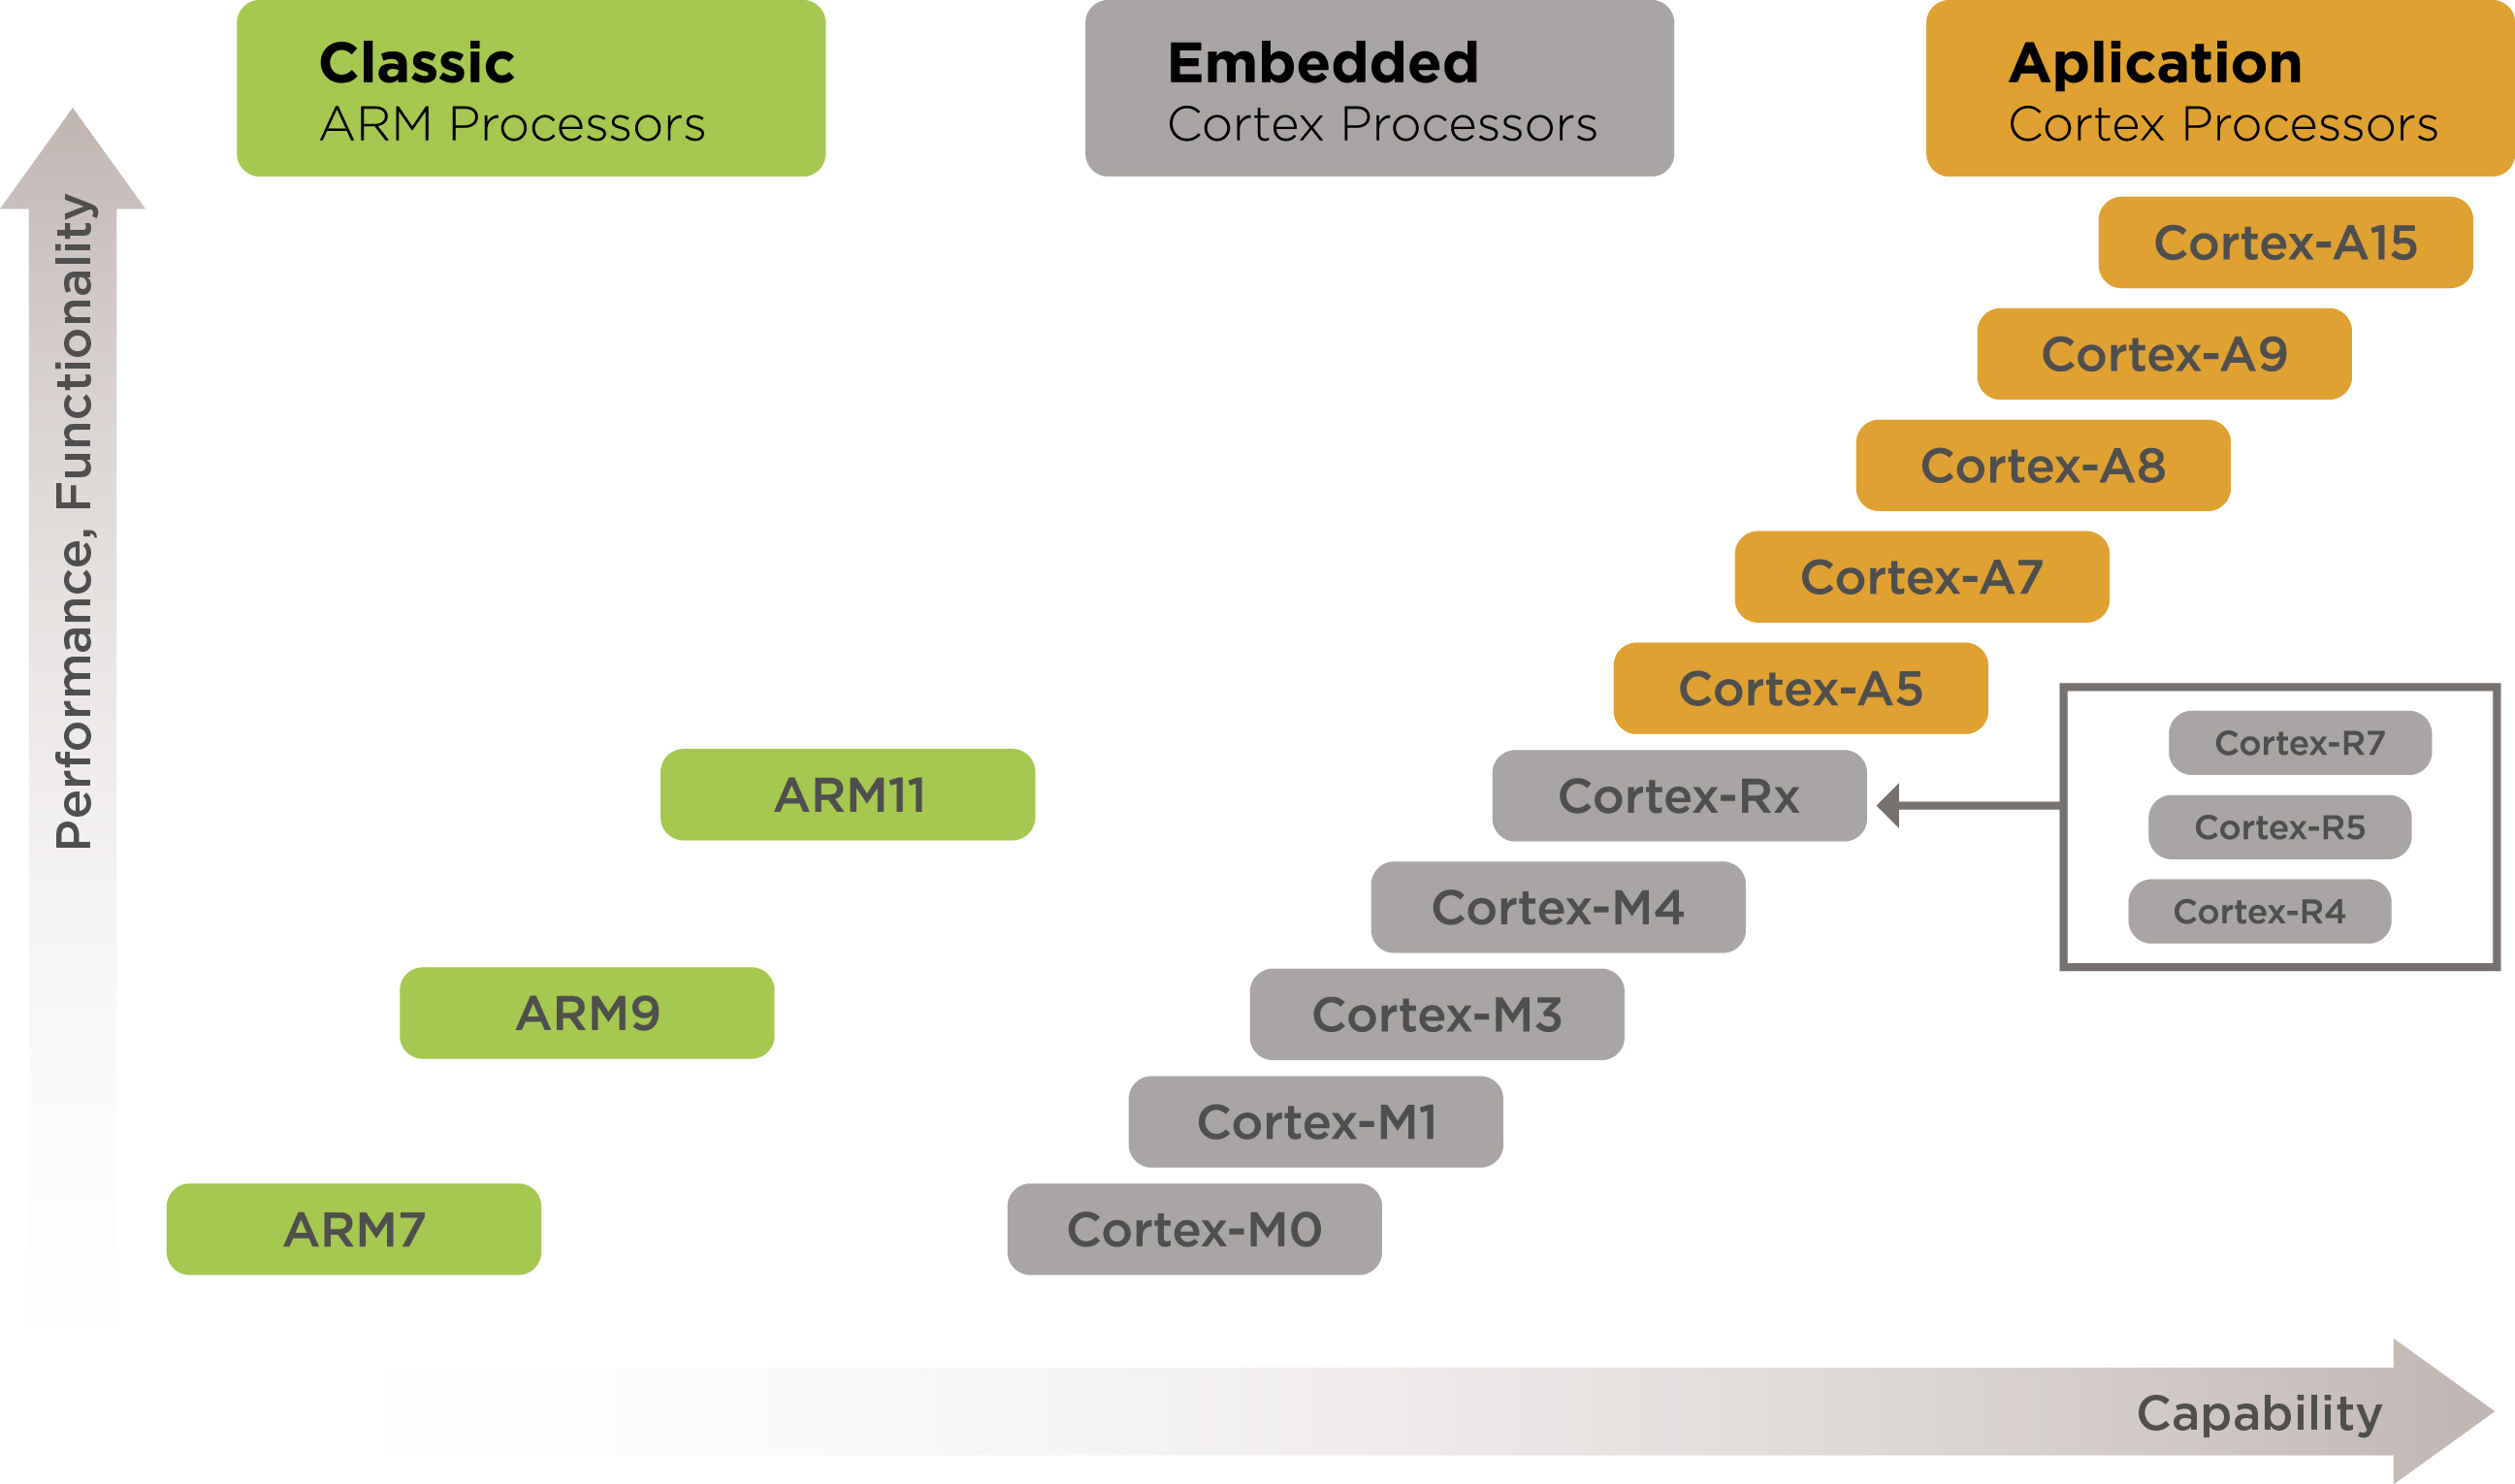
\includegraphics[width=0.8\textwidth]{images/all-arm.jpg}
    \caption{Các dòng vi xử lý lõi ARM}
    \label{fig:all-arm-core}
\end{figure}
\subsection{Lõi ARM Cortex-M3}
\paragraph{}
Dòng ARM Cortex là một bộ xử lý thế hệ mới đưa ra một kiến trúc chuẩn cho nhu cầu đa dạng về công nghệ. Không giống như các chip ARM khác, dòng Cortex là một lõi xử lý hoàn thiện, đưa ra một chuẩn CPU và kiến trúc hệ thống chung. Dòng Cortex có ba phân nhánh chính:
\begin{itemize}
    \item Cấu hình A: cho các ứng dụng Application, yêu cầu cao chạy trên các hệ điều hành mở và phức tạp như Linux, Android.
    \item Cấu hình R: cho các ứng dụng thời gian thực Real Time.
    \item Cấu hình M: cho các ứng dụng \acrfull{mcu} Microcontroller.
\end{itemize}
\paragraph{}
Bộ vi xử lý ARM Cortex-M3 là bộ vi xử lý ARM đầu tiên dựa trên kiến trúc ARMv7-M và được thiết kế đặc biệt để đạt được hiệu suất cao trong các ứng dụng nhúng cần tiết kiệm năng lượng và chi phí, chẳng hạn như các vi điều khiển, hệ thống cơ ô tô, hệ thống kiểm soát công nghiệp và hệ thống mạng không dây. Thêm vào đó là việc lập trình được đơn giản hóa đáng kể giúp kiến trúc ARM trở thành một lựa chọn tốt cho ngay cả những ứng dụng đơn giản nhất.
\subsection{Dòng vi điều khiển STM32}
\paragraph{}
STM32 là dòng vi điều khiển dựa trên một số lõi ARM Cortex-M 32 bit khác nhau\cite{stm32-types}. STMicroelectronics lấy bản quyền các vi xử lý được thiết kế bởi ARM Holdings với rất nhiều lựa chọn cấu hình và chọn ra các cấu hình cho từng thiết kế vi điều khiển của họ.


\begin{table}
    \centering
    \caption{Các dòng vi điều khiển STM32 và lõi ARM tương ứng}
    \begin{tabular}{|c|c|}
    \hline
    STM32 series & ARM CPU core(s) \\
    \hline
    F0 & Cortex-M0 \\
    \hline
    C0, G0, L0 & Cortex-M0+\\
    \hline
    F1, F2, L1 & Cortex-M3\\
    \hline
    F3, F4, G4, L4, L4+ & Cortex-M4\\
    \hline
    WB, WL & Cortex-M4, Cortex-M0+\\
    \hline
    F7 & Cortex-M7\\
    \hline
    H7 & Cortex-M7, Cortex-M4 \\
    \hline
    H5, L5, U5, WBA & Cortex-M33 \\
    \hline
    \end{tabular}
\end{table}
\paragraph{}
STM32F103 thuộc họ F1 với lõi ARM Cortex M3 là vi điều khiển 32 bit, tốc độ tối đa là 72Mhz. Giá thành tương đối rẻ so với các loại vi điều khiển có chức năng tương tự. Mạch nạp cũng như công cụ lập trình khá đa dạng và dễ sử dụng.
\section{Mạch phát triển STM32F103C8T6 - Blue Pill}
\subsection{\Acrlong{mcu} STM32F103C8T6}
\paragraph{}
\Acrlong{mcu} STM32F103C8T6 thuộc dòng \acrshort{mcu} STM32F1xx của ST Microelectronics với nhân ARM 32-bit Cortex M3 72MHz với các thông số quan trọng trong bảng \ref{tab:specs}.
\begin{table}[H]
    \centering
    \caption{Các thông số quan trọng của \acrshort{mcu} STM32F103C8T6}
    \begin{tabular}{|c|c|}
        \hline
        \multicolumn{2}{|c|}{Bộ nhớ} \\
        \hline
        Bộ nhớ SRAM & 20k bytes \\
        \hline
        Bộ nhớ Flash & 64k bytes \\
        \hline
        \hline
        \multicolumn{2}{|c|}{Clock, reset và quản lý nguồn} \\
        \hline
        Điện áp hoạt động & 2.0v - 3.6v \\
        \hline
        Thạch anh ngoại chính & 4MHz - 20 MHz \\
        \hline
        Thạch anh RTC & 32.768Hz \\
        \hline
        Ngoại vi quản lý điện áp & POR, PDR, PVD \\
        \hline
        Chế độ & Ngủ, chờ, ngừng hoạt động \\
        \hline
         
    \end{tabular}
    \label{tab:specs}
\end{table}

\paragraph{}
\acrshort{mcu} STM32F103C8T6 có đa dạng các ngoại vi cho ứng dụng nhúng:
\begin{itemize}
    \item 2 bộ ADC 12 bit với 9 kênh cho mỗi bộ
    \begin{itemize}
        \item Khoảng giá trị chuyển đổi từ 0 – 3.6V.
        \item Lấy mẫu nhiều kênh hoặc 1 kênh.
        \item Có cảm biến nhiệt độ nội.
    \end{itemize}
    \item Hỗ trợ 9 kênh giao tiếp bao gồm:
    \begin{itemize}
        \item 2 bộ \acrshort{i2c}(SMBus/PMBus)
        \item 3 bộ USART(ISO 7816 interface, LIN, IrDA capability, modem control)
        \item 2 bộ SPI (18 Mbit/s)
        \item 1 bộ CAN interface (2.0B Active)
        \item USB 2.0 full-speed interface
    \end{itemize}
    \item 7 Timer cho các ngoại vi:
    \begin{itemize}
        \item 3 timer 16 bit hỗ trợ các mode IC/OC/PWM.
        \item 1 timer 16 bit hỗ trợ để điều khiển động cơ với các mode bảo vệ như ngắt input, dead-time..
        \item 2 watchdog timer.
        \item 1 SysTick timer 24 bit đếm xuống dùng cho các ứng dụng như hàm Delay.
    \end{itemize}
    \item 7 kênh DMA cho các ngoại vi như ADC, \acrshort{i2c}, SPI, UART.
\end{itemize}
\subsection{Mạch phát triển Blue Pill}
\paragraph{}
Blue Pill là một mạch phát triển đơn giản cho \acrlong{mcu} STM32F103C8. Blue Pill ra đầy đủ chân của vi điều khiển cùng với cổng giao tiếp USB, các chân gỡ lỗi SWD và các chân thiết lập khởi động. 
\begin{figure}[H]
    \centering
    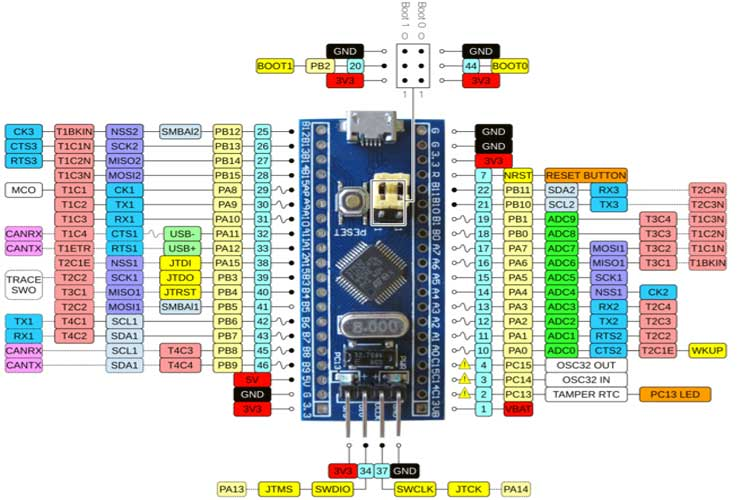
\includegraphics[width=0.9\textwidth]{images/STM32-Blue-Pill-Development-Board-Pinout.jpg}
    \caption{Ra chân của mạch phát triển Blue Pill}
    \label{fig:bluepill}
\end{figure}
Về chi tiết, mạch phát triển Blue Pill bao gồm:
\begin{itemize}
    \item \acrshort{mcu} STM32F103C8T6.
    \item Led báo trạng thái nguồn, led PC13, nút nhấn reset.
    \item IC chuyển đổi điện áp từ 5 xuống 3.3v cung cấp cho vi điều khiển.
    \item Cổng Micro USB kết nối tới ngoại vi USB của vi điều khiển và cấp nguồn.
    \item Thạch anh ngoại 8MHz.
    \item Thạch anh ngoại thời gian thực 32KHz.
    \item Ra chân đầy đủ tất cả GPIO và các giao tiếp \acrshort{i2c}, CAN, UART, SPI, USB, ...
\end{itemize}
\section{Lập trình cho mạch phát triển Blue Pill}
\subsection{Môi trường lập trình cho Blue Pill}
\paragraph{}
Mỗi \acrlong{mcu} dòng ARM lại có kiểu kiến trúc khác nhau. Đối với STM32 nói chung và STM32F103C8 được sử dụng trong Blue Pill, bộ công cụ lập trình GCC được sử dụng là arm-none-eabi-, đối với các ngôn ngữ rust, bộ công cụ được sử dụng là thumbv7m-none-eabi.
\paragraph{}
Để lập trình cho vi điều khiển STM32, các công cụ soạn thảo nên có những gợi ý cho người dùng, giúp người dùng có thể dễ dàng biên dịch và nạp cho thiết bị \acrlong{mcu}. Một số phần mềm có thể sử dụng bao gồm:
\begin{itemize}
    \item STM32CubeIDE và STM32CubeMX: Phần mềm chính hãng từ ST giúp thiết lập trước các thông số và soạn thảo phần mềm cho STM32. Có thể kết hợp với STM32CubeProg giúp nạp chương trình cho \acrlong{mcu}.
    \item $\mu$Vision IDE: Công cụ soạn thảo và gỡ lỗi hỗ trợ trực tiếp cho ARM.
    \item Công cụ soạn thảo khác như VSCode, Vim, Notepad++, ...: Các công cụ này thường không có sẵn môi trường phát triển cho STM32, cần thiết lập thêm qua các công cụ khác.
\end{itemize}
\subsection{Các thư viện lập trình}
\paragraph{}
Các thư viện lập trình sẽ giúp đơn giản hóa quá trình phát triển phần mềm cho các \acrlong{mcu}. Các thư viện hỗ trợ lập trình đã có sẵn và rất đa dạng, đang được sử dụng rộng rãi như thư viện từ ST, thư viện Arduino hay từ Rust.
\paragraph{}
Các thư viện được chia thành các mức khác nhau, từ cấp thấp đến cấp cao. Ở mức PAC, các thanh ghi của các thành phần ngoại vi được tích hợp vào thư viện giúp người lập trình có thể tương tác trực tiếp với các thành ghi. Tại mức HAL, các ngoại vi của vi điều khiển được trừu tượng hóa thành các kiểu dữ liệu của ngôn ngữ lập trình, giúp người lập trình có thể lập trình \acrlong{mcu} mà không cần hiểu chuyên sâu về các thanh ghi. Đối với mức Board, các thành phần mức HAL được tổng hợp lại, chỉnh sửa để hỗ trợ cho việc lập trình từ các mạch phát triển:
\begin{figure}[H]
    \centering
    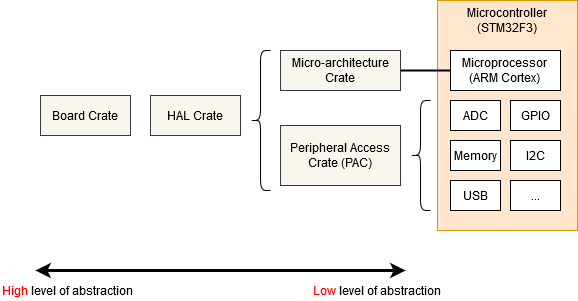
\includegraphics[width=0.8\textwidth]{images/crates.png}
    \caption{Các mức hỗ trợ của thư viện lập trình}
    \label{fig:embedded-library}
\end{figure}
\subsection{Nạp chương trình}
\paragraph{}
Sau khi đã phát triển chương trình cho STM32, chương trình sau khi biên dịch cần được nạp vào \acrshort{mcu} để chạy. Mạch phát triển Blue Pill hỗ trợ 2 phương thức nạp phần mềm phổ biến là UART qua ngoại vi UASRT1 sử dụng các thiết bị USB to UART và qua giao thức SWD sử dụng các thiết bị JLink, STLink hay SMSIS-DAP. Có một số phần mềm hỗ trợ nạp bằng cả 2 giao thức này:
\begin{itemize}
    \item STM32CubeProgrammer: Đây là công cụ chính hãng để nạp phần mềm cho các sản phẩm \acrlong{mcu} từ ST. Công cụ này hỗ trợ nhiều chuẩn giao tiếp khác nhau cùng nhiều chức năng nâng cao như đọc, ghi, xác thực chương trình hay tự động hóa quá trình nạp phần mềm.
    \item Probe-rs: Probe-rs là một bộ công cụ mới giúp gỡ lỗi cho thiết bị nhúng, giúp nạp chương trình cho các vi điều khiển ARM, RISC-V sử dụng các chuẩn nạp khác nhau như CMSIS-DAP, STLink, JLink. Ngoài ra, probe-rs còn hỗ trợ các chuẩn gỡ lỗi như GDB và Microsoft DAP giúp gỡ lỗi qua Visual Studio Code hoặc qua giao diện dòng lệnh.
\end{itemize}
\section{Giao tiếp USART}
\paragraph{}
UART là một ngoại vi cơ bản và thường dùng trong các quá trình giao tiếp với các module như: Xbee, Wifi, Bluetooth…Khi giao tiếp UART kết hợp với các IC giao tiếp như MAX232CP, SP485EEN… thì sẽ tạo thành các chuẩn giao tiếp RS232, RS485. Đây là các chuẩn giao tiếp thông dụng và phổ biến trong công nghiệp từ trước đến nay.
\paragraph{}
Giao tiếp USART yêu cầu chân GND chung, chân Tx, chân Rx và chân CLK tùy chọn. Khi sử dụng chân UART\_CLK thì giao tiếp UART sẽ trở thành giao tiếp đồng bộ và không dùng sẽ là chuẩn giao tiếp không đồng bộ:
\begin{figure}[H]
    \centering
    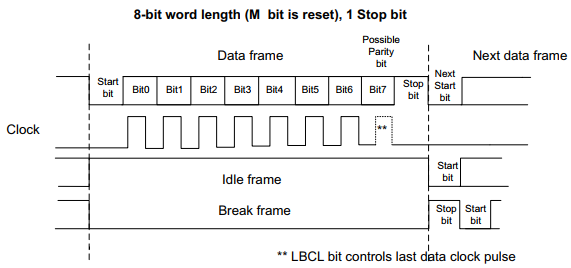
\includegraphics[width=0.8\textwidth]{images/uart-2.png}
    \caption{Giap tiếp USART}
    \label{fig:uart}
\end{figure}

\paragraph{}
Ưu điểm của giao tiếp UART không đồng bộ: tiết kiệm chân vi điều khiển (2 chân), là ngoại vi mà bất kì một vi điều khiển nào cũng có, có khá nhiều module, cảm biến dùng UART để truyền nhận data với vi điều khiển. 
\paragraph{}
Nhược điểm của loại ngoại vi này là tốc độ khá chậm, tốc độ tối đa tùy thuộc vào từng dòng, quá trình truyền nhận dễ xảy ra lỗi nên trong quá trình truyền nhận cần có các phương pháp để kiểm tra (thông thường là truyền thêm bit hoặc byte kiểm tra lỗi). UART không phải là một chuẩn truyền thông, khi muốn nó là một chuẩn truyền thông hoặc truyền data đi xa, cần phải sử dụng các IC thông dụng để tạo thành các chuẩn giao tiếp đáng tin cậy như RS485 hay RS232....
\paragraph{}
STM32F103C8 có 3 bộ UART với nhiều mode hoạt động với một số tính năng nổi bật như sau:
\begin{itemize}
    \item Đầy đủ các tính năng của bộ giao tiếp không đồng bộ.
    \item Điều chỉnh baud rate bằng lập trình và tốc độ tối đa lên đến 4.5Mb/s.
    \item Độ dài được lập trình là 8 hoặc 9 bit.
    \item Cấu hình bit stop hỗ trợ là 1 hoặc 2.
    \item Có chân clock nếu muốn chuyển giao tiếp thành đồng bộ.
    \item Cấu hình sử dụng 1 dây hoặc 2 dây.
    \item Có bộ DMA nếu muốn đẩy cao thời gian truyền nhận.
    \item Bit cho phép truyền nhận riêng biệt.
\end{itemize}

\paragraph{}
Thông thường sẽ dùng ngắt nhận UART để nhận dữ liệu vì sử dụng ngắt sẽ tiện lợi, không tốn thời gian chờ cũng như mất dữ liệu. Các tốc độ thường dùng để giao tiếp với máy tính: 600, 1200, 2400, 4800, 9600, 14400, 19200, 38400, 56000, 57600, 115200. 

\paragraph{}
Thực hiện kết nối giao tiếp UART bằng cách kết nối chân GND, Tx, Rx của thiết bị 1 với chân GND, Rx, Tx của thiết bị 2 (Hình \ref{fig:uart-wiring}).
\begin{figure}[H]
    \centering
    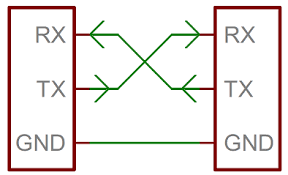
\includegraphics[width=0.6\textwidth]{images/Untitled.png}
    \caption{Kết nối chân giao tiếp UART}
    \label{fig:uart-wiring}
\end{figure}
\paragraph{}
Một số phần mềm giao tiếp với máy tính bao gồm: picocom(linux), Hercules\_3-2-5, teraterm, SerialOscilloscope-v1.5... Một số module dùng để giao tiếp với máy tính: CP2102 USB 2.0, module PL2303, module FT232RL, CH340G hoặc sử dụng mạch CMSIS-DAP tích hợp cả SWD và UART.

\section{Giao tiếp \acrshort{i2c}}
\paragraph{}
\acrfull{i2c} là một loại bus nối tiếp đồng bộ hai chiều với 2 dây tín hiệu. STM32F103C8T6 có hai bộ \acrshort{i2c} có thể lập trình được:
\begin{itemize}
    \item 2 chế độ Master và Slave
    \item Có thể lập trình địa chỉ cho chế độ Slave, có chế độ kiểm tra start/stop.
    \item Hỗ trợ chế độ địa chỉ 7 bit và 10 bit.
    \item Hỗ trợ hai chuẩn tốc độ 100Khz và 400 Khz.
    \item Có bộ lọc nhiễu Analog.
    \item Tích hợp mode DMA.
    \item Có các cờ báo trạng thái: Nhận, truyền, kết thúc chuyển đổi, báo lỗi.
    \item Có các ngắt như: Ngắt buffer truyền, nhận; ngắt sự kiện, ngắt báo lỗi.
    \item Quá trình truyền data tùy thuộc vào mode cấu hình của I2C là master hoặc slave, ở chế độ 10 bit địa chỉ hay 7 bit địa chỉ (phổ biến hơn).
\end{itemize}
\paragraph{}
Kết nối \acrshort{i2c} được thực hiện bằng cách kết nối các chân SDA và CLK của các thiết bị lại với nhau (Hình \ref{fig:i2c-wiring}).
\begin{figure}[H]
    \centering
    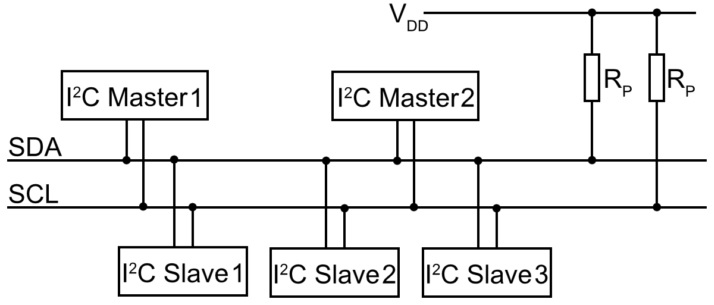
\includegraphics[width=0.8\textwidth]{images/I2C-Bus-Layout.jpg}
    \caption{Caption}
    \label{fig:i2c-wiring}
\end{figure}
\section{Module LCD1602 sử dụng ic HD44780}
\paragraph{}
HD44780 là một ic điều khiển màn hình ma trận điểm (dot-matrix) giúp hiển thị các ký tự chữ, số và các ký tự. Nó có thể được thiết lập để điều khiển với chế độ 4 bit hoặc 8 bit. Tất cả các chức năng như bộ nhớ hiển thị, bộ sinh ký tự hiển thị và các thành phần điều khiển màn hình được tích hợp sẵn trong một ic, vì vậy việc điều khiển màn hình ma trận điểm có thể được thực hiện một cách dễ dàng.

\begin{figure}[H]
    \centering
    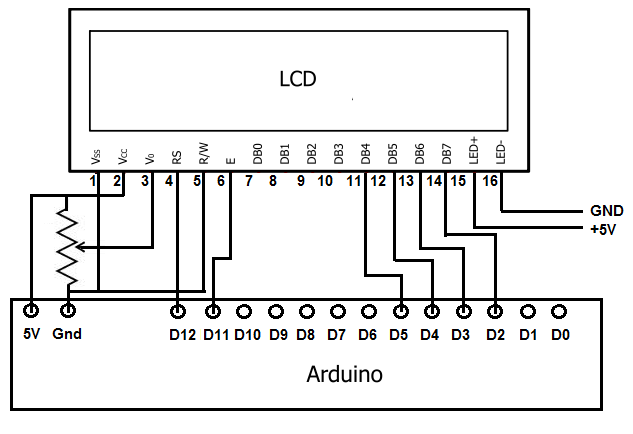
\includegraphics[width=0.8\textwidth]{images/Arduino-HD44780-circuit-schematic.png}
    \caption{Màn hình LCD1602 HD44780}
    \label{fig:hd44780}
\end{figure}
\paragraph{}
Một số chức năng có thể kể đến bao gồm:
\begin{itemize}
    \item Điện áp sử dụng: 2.V7-5.5V
    \item Bộ nhớ tối đa: 80 ký tự
    \item Có một số chức năng như: Xóa màn hình, quay về đầu, bật tắt hiển thị, bật tắt con trỏ, bật tắt nháy con trỏ, di chuyển con trỏ, di chuyển màn hình.   
    \item Đối với chế độ 4 bit, thực hiện ghi lần lượt 4 bit thấp và 4 bit cao cho một ký tự.
\end{itemize}

\begin{figure}[H]
    \centering
    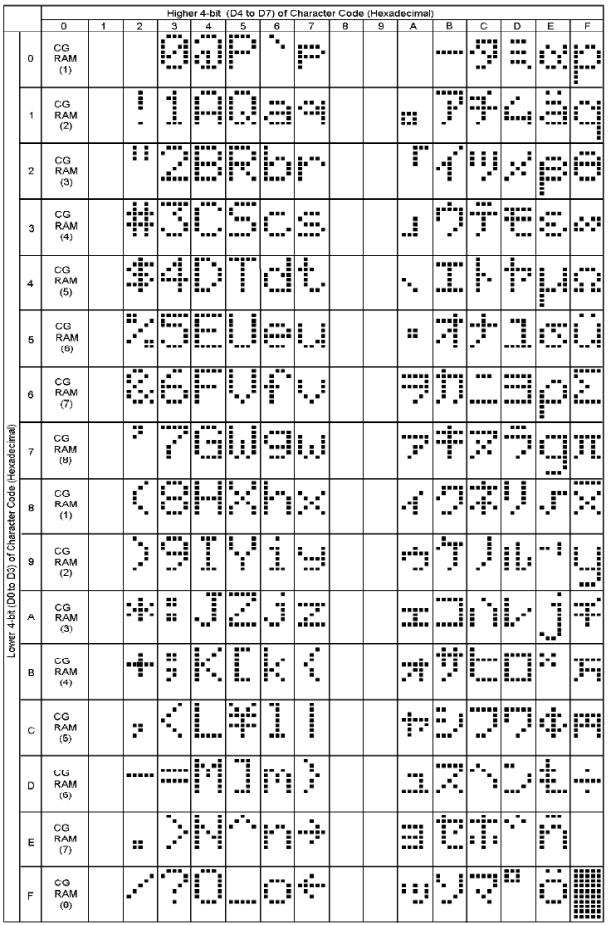
\includegraphics[width=0.8\textwidth]{images/Asciichart.png}
    \caption{Bảng ký tự điều khiển màn hình LCD1602}
    \label{fig:hd44780-char}
\end{figure}

\section{Module mở rộng I/O PCF8574}
\paragraph{}
Khi kết nối tới màn hình LCD1602, số lượng chân I/O cần thiết cho chế độ 4 bit là 6, và 10 tương ứng với chế độ 8 bit. Để tiết kiệm chân điều khiển và đơn giản hóa quá trình điều khiển, các module mở rộng chân sẽ là giải pháp tối ưu.
\paragraph{}
PCF8574 là một module mở rộng vào ra 8 bit sử dụng giao tiếp \acrshort{i2c} được sử dụng rộng rãi với 8 địa chỉ có thể thay đổi được. Với mỗi byte được ghi vào module qua giao tiếp \acrshort{i2c}, các bit tương ứng sẽ được bật tắt giúp điều khiển LCD1602.
\begin{figure}[H]
    \centering
    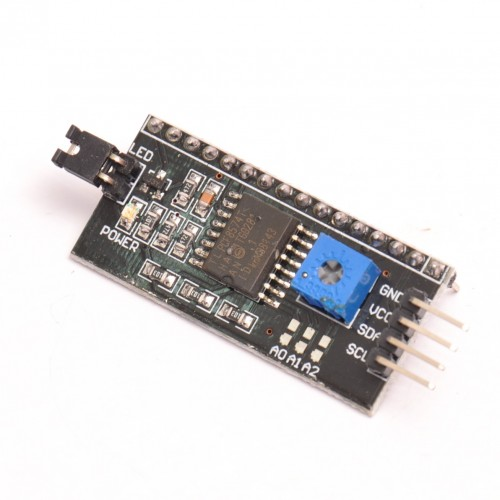
\includegraphics[width=0.8\textwidth]{images/I2C_PCF.jpg}
    \caption{Module PCF8574 cho màn hình LCD1602}
    \label{fig:pcf8574}
\end{figure}

\chapter{THỰC HIỆN ĐỀ TÀI}
\section{Yêu cầu hệ thống}
\paragraph{}
Hệ thống thiết bị phải được lắp đặt và lập trình cho các công việc sau:
\begin{itemize}
    \item Khi cấp nguồn thực hiện truyền dòng chữ "Họ và tên sinh viên là: " lên màn hình console của máy tính qua giao tiếp uart.
    \item Khi người dùng gõ các ký tự lên màn hình console, dữ liệu được gửi sang thiết bị và hiển thị trên màn hình LCD1602 cũng như gửi lại ký tự lên màn hình console để hiển thị cho người gõ.
    \item Nếu ký tự người dùng gõ không phải ký tự chữ cái, chữ số, dấu cách hoặc ký tự xuống dòng, bỏ qua ký tự.
    \item Nếu người dùng nhấn "Enter", thực hiện gửi chuỗi "Đã nhập: " và chuỗi người dùng nhập vào lên màn hinh máy tính, hiển thị trên màn hình LCD1602 dòng chữ "TEN SINH VIEN LA" và dòng 2 là chuỗi người dùng nhập.
    \item Nếu người dùng nhấn Enter sau lần nhấn Enter trước đó, thiết bị gửi chuỗi xóa màn hình console và gửi dòng "Họ và tên sinh viên là: " lên màn hình console của máy tính. Khi người dùng nhập ký tự đầu tiên, thực hiện xóa màn hình LCD1602 và thực hiện in ký tự đó và các ký tự tiếp theo.
\end{itemize}

\paragraph{}
Một số yêu cầu phi chức năng khác:
\begin{itemize}
    \item Hệ thống cần đáp ứng nhanh, xử lý nhanh tránh trường hợp người dùng cảm nhận được độ trễ khi nhập.
    \item Khi người dùng nhập ký tự nhanh (từ 20ms), không được làm mất ký tự.
    \item Nhận đúng ký tự người dùng nhập vào và hiển thị đúng ký tự đó lên màn hình console cũng như màn hình LCD1602.
    \item Số ký tự tối đa được nhập dưới 100 ký tự, nếu vượt quá khoảng hiển thị của màn hình LCD1602, thực hiện thuật toán cuộn trang để hiển thị các ký tự.
\end{itemize}
\section{Lựa chọn và lắp đặt phần cứng}
\subsection{Sơ đồ phần cứng}
Đối với phần cứng, kết nối giữa module \acrshort{i2c} và \acrlong{mcu} được thực hiện như trong bảng \ref{tab:lcd-wiring} để sử dụng ngoại vi I2C1.

\begin{table}[H]
    \centering
    \caption{Chân kết nối màn hình LCD}
    \begin{tabular}{|c|c|}
        \hline
        Chân vi điều khiển & Chân module \acrshort{i2c} \\
        \hline
        PB8 (SDA) & SDA \\
        \hline
        PB9 (CLK) & CLK \\
        \hline
        GND & GND \\
        \hline
    \end{tabular}
    \label{tab:lcd-wiring}
\end{table}

\paragraph{}
Thiết bị chuyển USB sang UART được sử dụng là module CMSIS-DAP, tích hợp sẵn khả năng nạp chương trình qua chuẩn SWD và chuyển đổi USB sang UART. Sau khi kết hối các thiết bị, ta có sơ đồ như trong hình \ref{fig:dev-block}.

\begin{figure}[H]
    \centering
    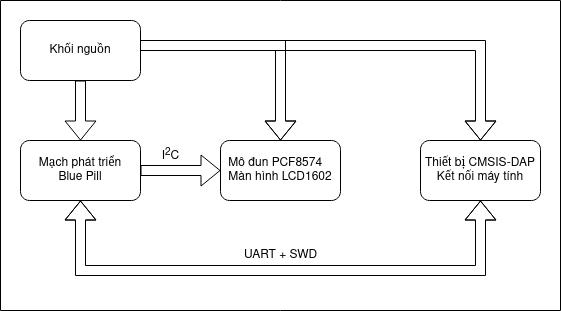
\includegraphics[width=0.8\textwidth]{images/arm-co-ban-device-block-diagram.drawio.png}
    \caption{Sơ đồ các thiết bị của hệ thống}
    \label{fig:dev-block}
\end{figure}
\subsection{Phần cứng thực tế sau khi ghép nối}

\section{Các thành phần phần mềm}

\subsection{Lựa chọn công cụ phát triển}
Rust là một ngôn ngữ lập trình mới có triển vọng trong nhiều lĩnh vực trong đó có lĩnh vực lập trình cho thiết bị nhúng. Vì vậy, nhóm quyết định phát triển hệ thống bằng ngôn ngữ này. Ứng dụng cho mảng nhúng, một số điểm mạnh của ngôn ngữ Rust bao gồm:
\begin{itemize}
    \item Hệ thống kiểu dữ liệu mạnh mẽ giúp tránh các lỗi liên quan đến bộ nhớ cũng như về luồng. Giúp chương trình chạy an toàn và dễ dàng đúng với mong muốn đặt ra hơn. Ví dụ như trong quản lý ngắt, luồng ngắt và luồng chính sẽ không thể gây ra sai xót về dữ liệu khi sử dụng Rust.
    \item Dữ liệu được quản lý an toàn mà không yêu cầu trình dọn rác. Điều này đặc biệt quan trọng do các thiết bị nhúng thường có cấu hình không cao.
    \item Các thư viện mã nguồn mở đa dạng, thân thiện với người dùng hơn nhờ hệ thống kiểu dữ liệu đa dạng, có thể tích hợp các phương thức giống lập trình hướng đối tượng trong khi vẫn đảm bảo các chức năng cấp thấp cần thiết cho lập trình nhúng.
    \item Trình biên dịch mạnh mẽ, giúp phát hiện lỗi ngay từ khi lúc biên dịch. Khi chương trình biên dịch thành công là chương trình có thể hoạt động được. Lỗi logic không thể được phát hiện nên cần được kiểm tra kỹ.
\end{itemize}

\paragraph{}
Môi trường phát triển dựa trên trình soạn thảo Neovim có tích hợp công cụ rust-analyzer cho việc lập trình Rust. Công cụ gỡ lỗi sử dụng probe-run giúp quá trình phát triển dễ dàng hơn.
\begin{figure}[H]
    \centering
    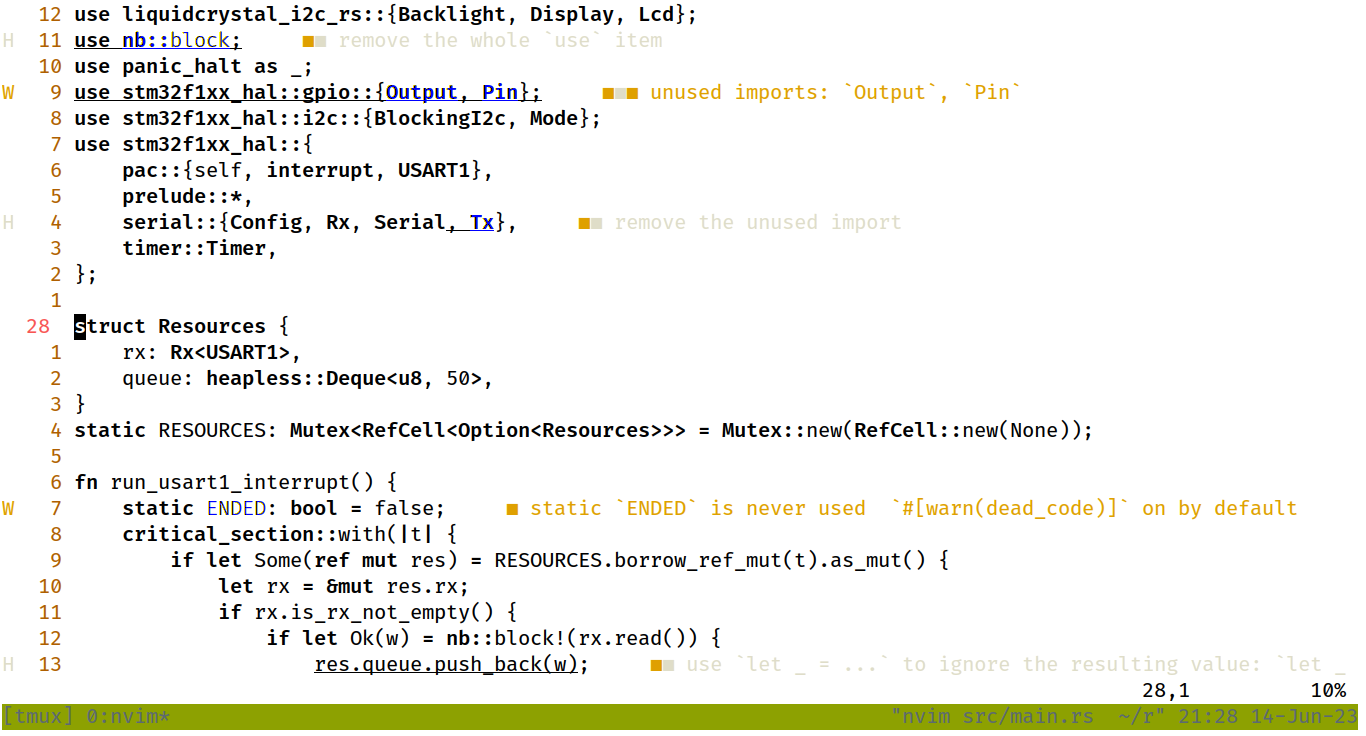
\includegraphics[width=0.8\textwidth]{images/Screenshot from 2023-06-14 21-28-38.png}
    \caption{Môi trường lập trình trên Neovim và rust-analyzer}
    \label{fig:neovim-environment}
\end{figure}


\subsection{Lựa chọn các thư viện}
\paragraph{}
Các thư viện cần thiết khi lập trình cho thiết bị nhúng bao gồm thư viện hỗ trợ phần cứng HAL và các thư viện đặc biệt giúp thao tác với các thiết bị ngoại vi được gắn thêm. Ngoài ra, các phần mềm 
\subsection{Triển khai phần mềm}

\section{Đánh giá}

\subsection{Kết quả đạt được}
Hệ thống đã đảm bảo đầy đủ theo các chức năng như đề ra trong đề tài. Hệ thống đã được xây dựng với các thiết bị phần cứng và phần mềm đúng như yêu cầu môn học đưa ra.
Thời gian hiển thị tương đối chính xác theo giờ tiêu chuẩn.

\subsection{Hạn chế của hệ thống}
Hệ thống đã đạt được mong muốn đề ra nhưng cũng không tránh khỏi những sai sót. Do hệ thống được phát triển ở mức thực nghiệm nên thiết kế sản phẩm có sơ sài về mặt kết nối các phần cứng. Đôi khi kết nối chập chờn dẫn đến sai sót trong hiển thị.


\chapter{KẾT LUẬN}
\section{Kết quả đạt được}
\section{Hướng phát triển và đề xuất}

\renewcommand\bibname{TÀI LIỆU THAM KHẢO}

\bibliographystyle{plain}

\printglossary[title=TỪ VIẾT TẮT, toctitle=DANH SÁCH TỪ VIẾT TẮT, type=\acronymtype]

\bibliography{refs}

\end{document}